%!TEX root = paper.tex

\begin{figure}[t]
\begin{subfigure}[t]{0.9\columnwidth}
\begin{center}
 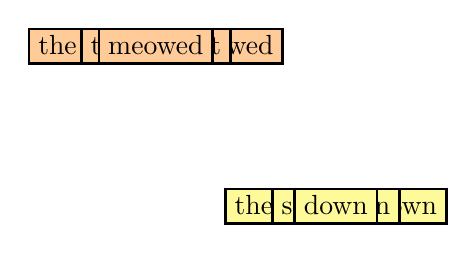
\begin{tikzpicture}
    \tikzstyle{word}=[fill=yellow!40,text height=2mm,line width=1pt,draw=black]    
    \tikzstyle{nonleaf}=[fill=yellow!40,text height=2mm,line width=1pt,draw=black]
    \tikzstyle{alt}=[fill=orange!40]    
    \pgfsetarrowsend{latex}
    \tikzset{edge from parent/.append style={<-, line width=1pt}}   

    \begin{scope}[shift={(0in,0in)}]

    \Tree [.\node[nonleaf,alt](2thekittenmeowed){the old cat meowed}; [.\node[nonleaf,alt](2thekitten){the old cat}; \node[word,alt](2the){the}; [.\node[nonleaf,alt](2bigkitten){old cat}; \node[word,alt](2kitten){old}; \node[word,alt](2kitten){cat}; ] ] \node[word,alt](2meowed){meowed}; ]

    \end{scope}


    \begin{scope}[shift={(0.9in,-0.8in)}, frontier/.style={distance from root=60pt}]

    \Tree [.\node[nonleaf](1thecatsatdown){the cat sat down}; [.\node[nonleaf](1thecat){the cat}; \node[word](1the){the}; \node[word](1cat){cat}; ] [.\node[nonleaf](1satdown){sat down}; \node[word](1sat){sat}; \node[word](1down){down}; ] ]

    \end{scope}

\end{tikzpicture}
\end{center}

\caption{\label{fig:batching:bad}Trees are hard to batch.}
\end{subfigure}

\vspace{2em}

\begin{subfigure}[t]{0.9\columnwidth}
 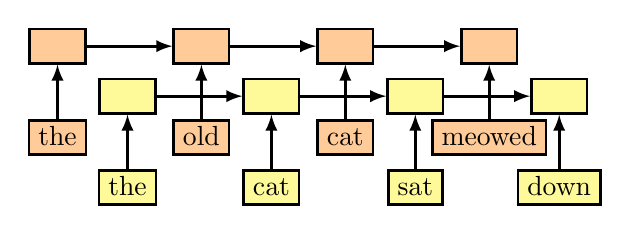
\begin{tikzpicture}
    \tikzstyle{word}=[fill=yellow!40,text height=2mm,line width=1pt,draw=black]    
    \tikzstyle{nonleaf}=[fill=yellow!40,text height=2mm,line width=1pt,draw=black] 
    \tikzstyle{alt}=[fill=orange!40]
    \pgfsetarrowsend{latex}
    \tikzstyle{fwd} = [draw=black, line width=1pt]
   
    \def\dx{26pt}
    \def\dy{11pt}
    \def\sy{7*\dy}
    \def\oxb{5.5*\dx}
    \def\by{1*\dy}
    \def\ox{0*\oxb}


    \begin{scope}[shift={(0in,0in)}, frontier/.style={distance from root=60pt}]
    
    \node[word,alt]  (w1) at (\ox+-3*\dx,\by+0*\dy) {the};
    \node[word,alt]  (w2) at (\ox+-1*\dx,\by+0*\dy) {old};
    \node[word,alt]  (w3) at (\ox+1*\dx,\by+0*\dy) {cat};
    \node[word,alt]  (w4) at (\ox+3*\dx,\by+0*\dy) {meowed};

    \node[word,alt]  (n1) at (\ox+-3*\dx,\by+3*\dy) {~~~~~};
    \node[word,alt]  (n2) at (\ox+-1*\dx,\by+3*\dy) {~~~~~};
    \node[word,alt]  (n3) at (\ox+1*\dx,\by+3*\dy) {~~~~~};
    \node[word,alt]  (n4) at (\ox+3*\dx,\by+3*\dy) {~~~~~};

   \draw [fwd] (w1) -- (n1);
   \draw [fwd] (w2) -- (n2);
   \draw [fwd] (w3) -- (n3);
   \draw [fwd] (w4) -- (n4);

   \draw [fwd] (n1) -- (n2);
   \draw [fwd] (n2) -- (n3);
   \draw [fwd] (n3) -- (n4);

    \end{scope}

    \begin{scope}[shift={(0.35in,-0.25in)}, frontier/.style={distance from root=60pt}]
    
    \node[word]  (w1) at (\ox+-3*\dx,\by+0*\dy) {the};
    \node[word]  (w2) at (\ox+-1*\dx,\by+0*\dy) {cat};
    \node[word]  (w3) at (\ox+1*\dx,\by+0*\dy) {sat};
    \node[word]  (w4) at (\ox+3*\dx,\by+0*\dy) {down};

    \node[word]  (n1) at (\ox+-3*\dx,\by+3*\dy) {~~~~~};
    \node[word]  (n2) at (\ox+-1*\dx,\by+3*\dy) {~~~~~};
    \node[word]  (n3) at (\ox+1*\dx,\by+3*\dy) {~~~~~};
    \node[word]  (n4) at (\ox+3*\dx,\by+3*\dy) {~~~~~};

   \draw [fwd] (w1) -- (n1);
   \draw [fwd] (w2) -- (n2);
   \draw [fwd] (w3) -- (n3);
   \draw [fwd] (w4) -- (n4);

   \draw [fwd] (n1) -- (n2);
   \draw [fwd] (n2) -- (n3);
   \draw [fwd] (n3) -- (n4);

    \end{scope}

\end{tikzpicture}


\caption{\label{fig:batching:good}Sequences are easy to batch.}
\end{subfigure}
\caption{An illustration of a conventionally-implemfented TreeRNN model (a) and a sequence-based RNN model (b).}
\end{figure}
